\documentclass[12pt]{amsart}
\setlength{\parskip}{.1in}
\setlength{\parindent}{0cm}
%myalterations
\usepackage{amssymb}
\usepackage{amsmath}
\usepackage[usenames,dvipsnames,svgnames,table]{xcolor}
\usepackage[colorlinks=true,urlcolor=blue,pdfborder={0 0 .5}pdfnewwindow=true]{hyperref}
\usepackage{enumitem}
%\usepackage{amsthm}
\usepackage{graphicx}
\usepackage{verbatim}
\usepackage{tabularx}
%\usepackage{arydshln,leftidx,mathtools}
\usepackage{bm}
\usepackage{tikz}
\usepackage{tikz-cd}
\usepackage{hyperref}
\usepackage{bm}

%\setlength{\dashlinedash}{.4pt}
%\setlength{\dashlinegap}{.8pt}
%\usepackage{amsthm}
\usepackage{verbatim}
%\usepackage{commath}
%My commands
%environment abbreviations
\newcommand{\benu}{\begin{enumerate}}
\newcommand{\eenu}{\end{enumerate}}
\newcommand{\bed}{\begin{description}}
\newcommand{\ed}{\end{description}}
\theoremstyle{definition}
\newtheorem{theorem}{Theorem}
\newtheorem{notation}[theorem]{Notation}
\newtheorem{exercise}[theorem]{Exercise}
\newcommand{\bex}{\begin{exercise}}
\newcommand{\ex}{\end{exercise}}

%symbol definitions
\newcommand{\un}[1]{\underline{#1}}
\newcommand{\mbZ}{\mathbb{Z}}
\newcommand{\mbR}{\mathbb{R}}
\newcommand{\mbN}{\mathbb{N}}
\newcommand{\mbQ}{\mathbb{Q}}
\newcommand{\mbC}{\mathbb{C}}
\newcommand{\mbF}{\mathbb{F}}
\newcommand{\mcS}{\mathcal{S}}
\newcommand{\mcP}{\mathcal{P}}
\newcommand{\hra}{\hookrightarrow}
\newcommand{\tra}{\twoheadrightarrow}
\newcommand{\lra}{\leftrightarrow}
\newcommand{\ep}{\epsilon}
\newcommand{\Ra}{\Rightarrow}
\newcommand{\mb}[1]{\mathbb{#1}}
\newcommand{\mc}[1]{\mathcal{#1}}
\newcommand{\bfs}[1]{{\bfseries #1}}
\newcommand{\bs}[1]{\boldsymbol{#1}}
%Operator definitions
\DeclareMathOperator{\Irr}{Irr}
\DeclareMathOperator{\triv}{triv}
\DeclareMathOperator{\cyc}{cyc}
\DeclareMathOperator{\lcm}{lcm}
\DeclareMathOperator{\expo}{x}
\DeclareMathOperator{\ord}{o}
\DeclareMathOperator{\imm}{im}
\DeclareMathOperator{\sgn}{sgn}
\DeclareMathOperator{\Sym}{Sym}
\DeclareMathOperator{\alt}{alt}
\DeclareMathOperator{\irr}{irr}
\DeclareMathOperator{\eqt}{Equiv}
\DeclareMathOperator{\pat}{Part}
%\DeclareMathOperator{\sgn}{sgn}
%\DeclareMathOperator{\Aut}{Aut}
\DeclareMathOperator{\Gl}{Gl}
\DeclareMathOperator{\M}{M}
\DeclareMathOperator{\Id}{Id}
\DeclareMathOperator{\fixx}{Fix}
\DeclareMathOperator{\suppp}{Supp}
\DeclareMathOperator{\gl}{Gl}
\DeclareMathOperator{\id}{Id}
\DeclareMathOperator{\Aut}{Aut}
\DeclareMathOperator{\Inn}{Inn}
\DeclareMathOperator{\orb}{orb}
\DeclareMathOperator{\ii}{I}
\DeclareMathOperator{\im}{im}
\DeclareMathOperator{\Fix}{Fix}
\DeclareMathOperator{\Co}{Co}
\DeclareMathOperator{\md}{md}
\DeclareMathOperator{\qt}{qt}
\DeclareMathOperator{\ExtendedGCD}{ExtendedGCD}
\DeclareMathOperator{\Mod}{Mod}
\DeclareMathOperator{\GCD}{GCD}
\newcommand{\nms}{\negmedspace}
\newcommand{\nts}{\negthinspace}

\newcommand{\itep}{\item {\bfseries Problem}\ }
\newcommand{\gen}[1]{\langle \nts#1 \nts\rangle}
\newcommand{\quot}[2]{#1/ #2}
\newcommand{\order}[1]{\left|<\nts #1 \nts s>\right|}

%These next two commands are for making answers. 
\newcommand{\beans}{\begin{description} \item[{ \bfseries \textcolor{red}{Answer}}]\ }
\newcommand{\eans }{\end{description}}
%\newcommand{\begin{comment}ex}{{ \bfseries \textcolor{red}{Answer}}}

%To turn the answer into problem sets use replace to replace \begin{comment} with \begin{comment} and \\end{comment}  by \end{comment}.
\newcommand{\lieb}[3][{{}}]{\frac{d^#1 #2}{d\,#3^#1}}

\title{\textbf{Math 521 - Problem Set 1}}
\author{Guy Matz}
\date{\today}

\begin{document} 

\maketitle
\newpage % Q1

\begin{enumerate}[series=p]
\itep 1
\\
Prove that for all set $A, B, C$ the formula
$$A \cup (B \cap C) = (A \cup B) \cap (A \cup C)$$
is true.
\\
$\Rightarrow$ We want to show that $A \cup (B \cap C) \subseteq (A \cup B) \cap (A \cup C)$.  That is, an arbitrary element, $x \in A \cup (B \cap C)$ is also in $(A \cup B) \cap (A \cup C)$.  Let $x \in A \cup(B \cap C)$.  Then either $x \in A$ or $x$ is in both $B$ and $C$.  So $x \in A$ or ($x \in B$ and $x \in C$).  Then we have ($x \in A$ or $x \in B$) and ($x \in A$ or $x \in C$), and therefore $x \in (A \cup B) \cap (A \cup C)$
\\\\
$\Leftarrow$ We want to show that $(A \cup B) \cap (A \cup C) \subseteq A \cup (B \cap C)$.  That is, an arbitrary element, $x \in (A \cup B) \cap (A \cup C)$ is also in $A \cup (B \cap C)$.  Let $x \in (A \cup B) \cap (A \cup C)$.  Then $x$ is in both $A$ and $B$ or $x$ is in both $A$ and $C$.  So $x$ is in $A$ or $x$ is in both $B$ and $C$, hence $x \in A \cup (B \cap C)$
\newpage % Q2

\itep 2
\benu
\item Prove that $(A^c)^c = A$
\\
$\Rightarrow$ We want to show that $(A^c)^c \subseteq A$\\
Let $x \in (A^c)^c$.  So $x \notin (A^c)$. Hence $x \in A$. 
\\
$\Leftarrow$ We want to show that $A \subseteq (A^c)^c$\\
Let $x \in A$.  So $x \notin (A^c)$. Hence $x \in (A^c)^c$. 
\\
\item Prove deMorgan's Law: $(A \cap B)^c = A^c \cup B^c$ and derive from the law $(A \cup B)^c = A^c \cap B^c$.
\\
$\Rightarrow$ We want to show that $(A \cap B)^c \subseteq A^c \cup B^c$.  Let $x \in (A \cap B)^c$.  Then $x \notin (A \cap B)$, so $x \notin A$ or $x \notin B$.  Hence $x \in A^c$ or $x \in B^c$, i.e. $x \in (A^c \cup B^c)$ 
\\\\
$\Leftarrow$ We want to show that $A^c \cup B^c \subseteq (A \cap B)^c$.  Let $x \in A^c \cup B^c$.  So $x \in A^c$ or $x \in B^c$.  Then $x \notin A$ or $x \notin B$, so $x \notin (A \cap B)$, i.e $x \in (A \cap B)^c$
\\
\\
How to derive $(A \cup B)^c = A^c \cap B^c$??
\begin{comment}
We can see that $(A \cup B)^c = A^c \cap B^c$ follows from above by setting $A' = A^c$ and $B' = B^c$. Then
$A' \cap B' = A^c \cap B^c$ and deMorgan’s law tells us that $(A' \cap B')^c = A'^c \cup B'^c = A \cup B$ . Taking the complement of both sets we see that $A' \cap B' = (A \cup B )^c$. Thus we have shown that $(A \cup B )^c = A^c \cap B^c$.
\end{comment}
\\
\item Draw Venn diagrams to illustrate the two laws
\\  THis isn't right, but how do I do this? \\
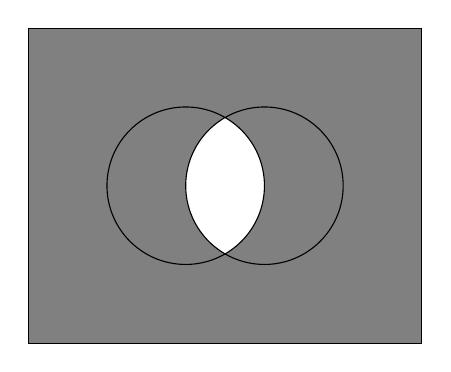
\begin{tikzpicture}
\filldraw[fill=gray] (-2,-2) rectangle (3,2);
\scope % A \cap B
\clip (0,0) circle (1);
\fill[white] (1,0) circle (1);
\endscope
% outline
\draw (0,0) circle (1)
(1,0) circle (1);
\end{tikzpicture}

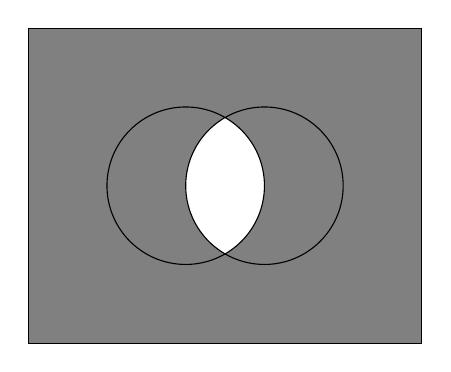
\begin{tikzpicture}
\filldraw[fill=gray] (-2,-2) rectangle (3,2);
\scope % A \cap B
\clip (0,0) circle (1);
\fill[white] (1,0) circle (1);
\endscope
% outline
\draw (0,0) circle (1)
(1,0) circle (1);
\end{tikzpicture}

\item Generalize these laws to more than two sets
\benu
\item $(A_1 \cap A_2 \cap \dots \cap A_n) = A_1^c \cup A_2^c \cup \dots \cup A_n^c$
\\
Induction on $n$\\
Base Step: See (b) above.
\\
Induction Hypothesis:
\\$(A_1 \cap A_2 \cap \dots \cap A_n) = A_1^c \cup A_2^c \cup \dots \cup A_n^c$
\\Induction Step:\\
$(A_1 \cap A_2 \cap \dots \cap A_{n+1}) = A_1^c \cup A_2^c \cup \dots \cup A_{n+1}^c$
IS THIS WHAT THEY'RE ASKING FOR?
\eenu

\eenu 

\newpage

\itep 3\\
Recast the following English sentences in mathematics, using correct mathematical grammar.  Preserve their meaning
\\
\benu
\item 2 is the smallest prime number
\\ Let $p \in \mathcal{P}$ where $\mathcal{P}$ is the set of all primes, $p \geq 2$
\item The area of any bounded plane region is bisected by some line parallel to the x-axis
\\
\\ ??
\\
\item All that glitters is not gold
\\Let $X$ be the set of all things that glitter, $Y$ be the set of all things that are gold.  $\exists x \in X$ such that $x \notin Y$
\eenu
\newpage

\itep 9\\
Let $x = A|B, x' = A'|B'$ be cuts in $\mbQ$.  We defined
$$x + x' = (A + A')|\text{ rest of } \mbQ$$
\benu
\item Show that although $B + B'$ is disjoint from $A + A'$, it may happen in degenerate cases that $\mbQ$ is not the union of $A + A'$ and $B + B'$
\\
Does "degenerate" is this case mean "lacking distinctness of structure usually present"?
\\

\item Infer that the definition of $x + x'$ as $(A + A')|(B + B')$ would be incorrect?
\\
What is this asking for?
\\
\item Why did we not define $x \cdot x' = (A \cdot A')|$rest of $\mbQ$?
\\
If either $x$ or $x'$ is negative, multiplication get "tricky".  See page 14-15
\eenu

\newpage
\itep 10\\
A multiplicative inverse of a non-zero cut $x = A|B$ is a cut $y = C|D$ such that $x \cdot y = 1$
\benu
\item If $x > 0^*$, what are $C$ and $D$?\\
\\
\item If $x < 0^*$, what are they?\\
\\
\item Prove that $x$ uniquely determines $y$
\eenu

\newpage
\itep 12\\
Let $b$ = l.u.b. $S$, where $S$ is a bounded nonempty subset  of $\mbR$.
\benu
\item Given $\epsilon > 0$ show that there exists an $s \in S$ with
$$b - \epsilon \leq s \leq b.$$
\\
\item Can $s \in S$ always be found so that $b - \epsilon < s < b$?
\\
\\
\item If $x = A|B$ is a cut in $\mbQ$, show that $x$ = l.u.b $A$.
\\
\\
\eenu

\newpage
\itep 13\\
Prove that $\sqrt{2} \in \mbR$ by showing that $x \cdot x = 2$ where $A|B$ is the cut in $\mbQ$ with $A = \{r = \mbQ: r \leq 0 \text{ or } r^2 < 2\}$.  Hint: Use exercise 12.

\newpage
\itep 14
Given $y \in \mbR, n \in \mbN,$ and $\epsilon > 0$, show that for some $\delta > 0$, if $u \in \mbR$ and $|u-y| < \delta$ then $|u^n - y^n| < \epsilon$.  Hint: Prove the inequality when $n = 1, n = 2$, and then do induction on n using the identity
$$u^n - y^n = (u-y)(u^{n-1} + u^{n-2}y + \dots + y^{n-1})$$.

\newpage
\itep 15
Given $x > 0$ and $n \in \mbN$, prove that there is a unique $y > 0$ such that $y^n = x$.  That is, $y = \sqrt[n]{x}$ exists and is unique.  Hint: Consider
$$y = \text{l.u.b.}\{s \in \mbR : s^n \leq x\}$$

\newpage
\item 16
Prove that real numbers correspond bijectively  to decimal expansions not terminating in an infinite strings of 9's, as follows.  The decimal expansion of $x \in \mbR$ is $N.x_1.x_2\dots$ where $N$ is the largest integer $\leq x, x_1$ is the largest integer $\leq 10(x-N), x_2$ is the largest integer $\leq 100(x-(N+x_1/10))$ and son on.
\\
\benu
\item Show that each $x_k$ is a digit between 0 and 9
\\
\item Show that for each $k$ there is an $l \geq k$ such that $x_l \neq 9$
\\
\item Conversely, show that for each such expression $N.x_1.x_2\dots$ not terminating in an infinite string of 9's, the set
$$ \{N, N + \frac{x_1}{10}, N + \frac{x_1}{10} + \frac{x_1}{100}\}$$
is bounded and its least upper bound is a real number $x$ with decimal expression $N.x_1.x_2\dots$
\\
\item Repeat the exercise with a general base in place of 10.
\eenu

\newpage
\itep *30\\
Suppose that a function $f : [a,b] \Rightarrow \mbR$ is monotone increasing i.e., $x_1 \leq x_2 \Rightarrow f(x_1) \leq f(x_2).$
\benu
\item Prove that $f$ is continuous except at a countable set of points.  [Hint: Show that at each $x \in (a,b), f$ has a right limit $f(x+)$ and a left limit $f(x-)$, which are limits of $f(x+h)$ as $h$ tends to 0 through positive, and negative values respectively.  The jump of $f$ at $x$ is $f(x+) - f(x-)$.  Show that $f$ is continuous at $x$ if and only if it has zero jump at $x$.  At how many points can $f$ have jump $\geq 1$?  At how many points can the jump be between 1/2 and 1?  Between 1/3 and 1/2?]
\\
\item Is the same assertion true for a monotone function defined on all of $\mbR$?
\\
\eenu

\newpage
\itep 36\\
A real number is algebraic if it is a root of a nonconstant polynomial with integer coefficients.
\benu
\item Prove that the set $A$ of algebraic numbers is denumerable.  [Hint: Each polynomial has how many roots?  How many linear polynomials are there?  How many quadratics? . . .]
\\
\\
\item Repeat the exercise for roots of polynomials whose coefficients belong to some fixed, arbitrary denumerable set $s \in \mbR$
\\
\\
\item Repeat the exercise for roots of trigonometric polynomials with integer coefficients.
\\
\\
\eenu

\end{enumerate}
\end{document}
